% !TEX encoding = UTF-8
% !TEX TS-program = pdflatex
% !TEX root = ../tesi.tex

%**************************************************************
\chapter{Progettazione e codifica}
\label{cap:progettazione-codifica}
%**************************************************************

La seguente sezione ha lo scopo di illustrare la soluzione ideata dal laureando per il soddisfacimento dei requisiti concordati con il tutor aziendale descritti nel capitolo \ref{cap:descrizione-stage}. Nella prima sezione viene presentato l'applicativo con il dovuto corredo di immagini, mentre nel secondo viene descritta accuratamente l'architettura implementata.


\section{L'applicativo SyncRec}
\subsection{Homepage}
\vspace{0.5em}
\begin{figure}[!h] 
	\centering 
	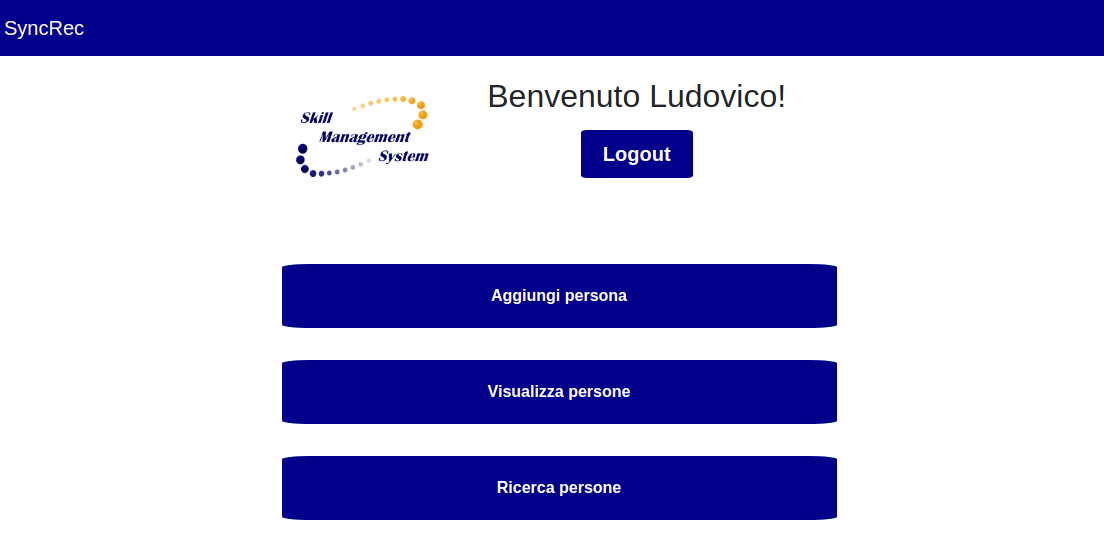
\includegraphics[width=1\columnwidth]{immagini/svil/homepage} 
	\caption{Schermata della homepage}
	\label{figura:homepage}
\end{figure}

\subsection{Maschera della visualizzazione degli\applicant}

\vspace{0.5em}
\begin{figure}[!h] 
	\centering 
	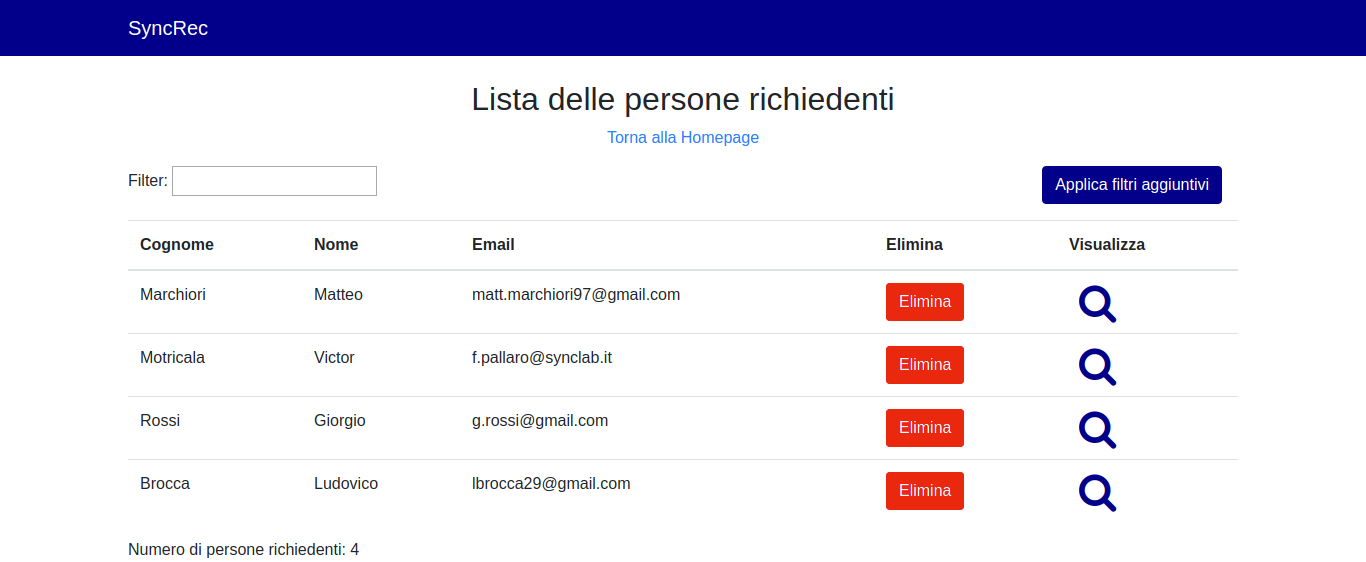
\includegraphics[width=1\columnwidth]{immagini/svil/lista} 
	\caption{Schermata della visualizzazione lista degli applicant}
	\label{figura:lista}
\end{figure}


\vspace{0.5em}
\begin{figure}[!h] 
	\centering 
	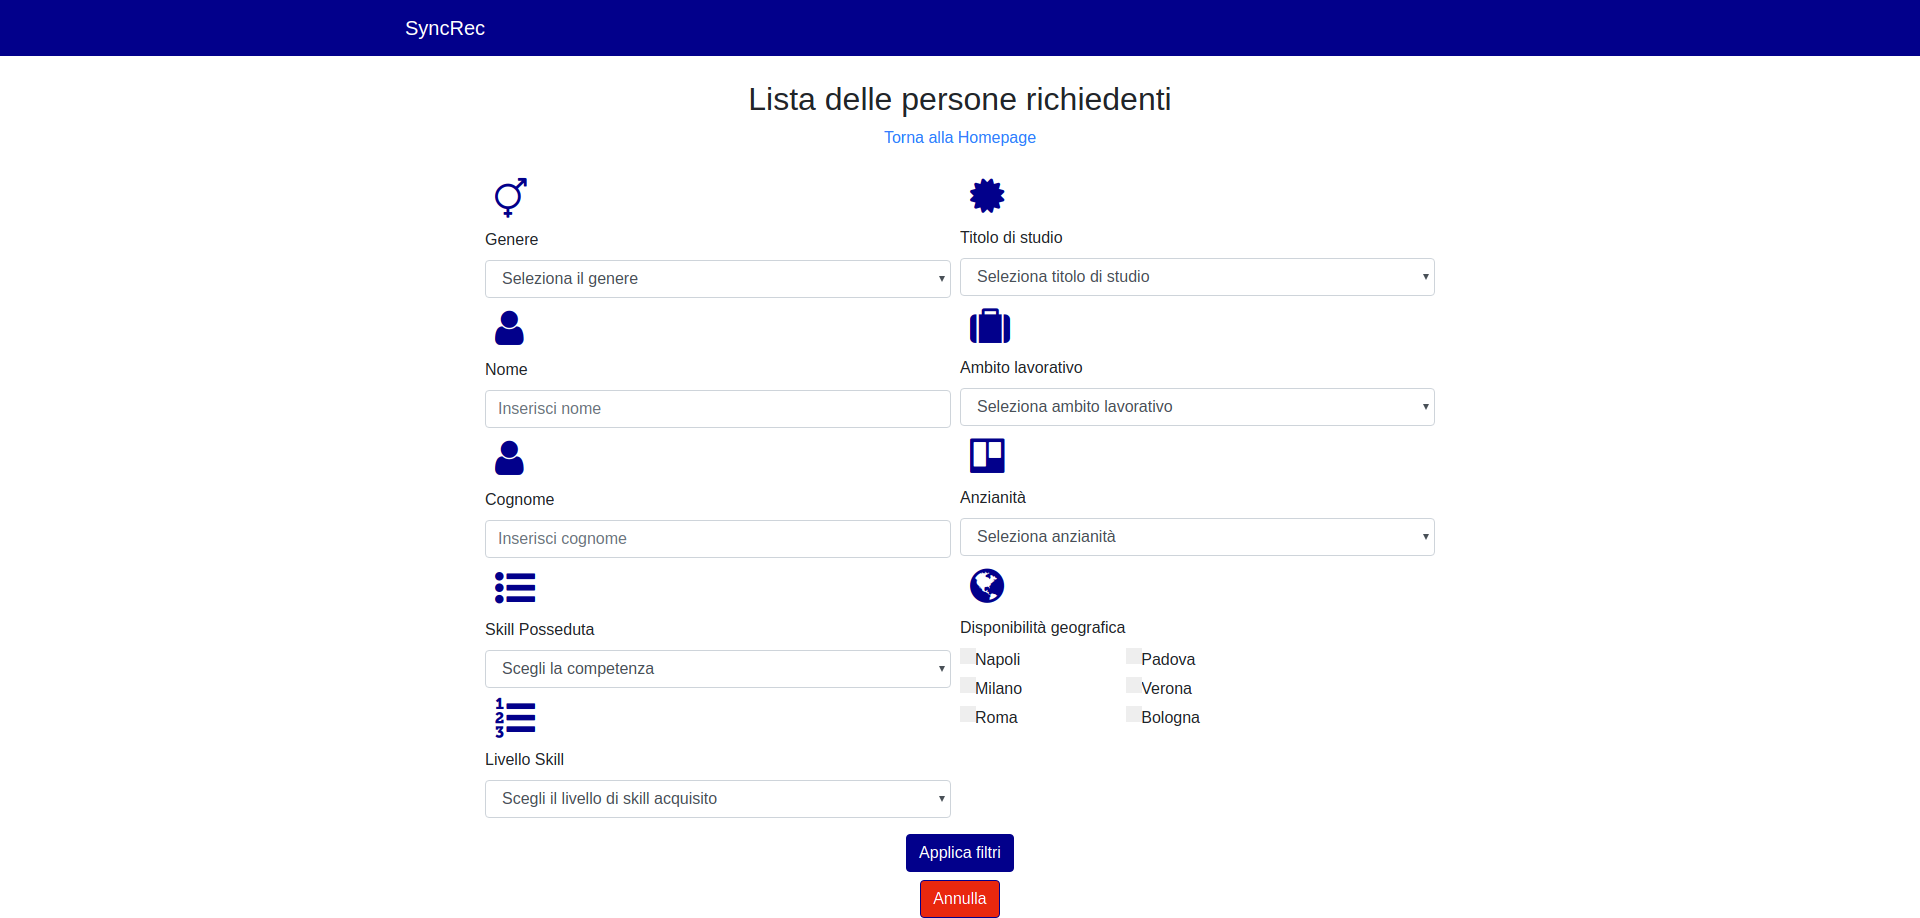
\includegraphics[width=1\columnwidth]{immagini/svil/filtri} 
	\caption{Schermata della selezione dei filtri da applicare alla lista degli applicant}
	\label{figura:filtri}
\end{figure}

\subsection{Maschera delle operazioni CRUD su un\applicant}
\vspace{0.5em}
\begin{figure}[!h] 
	\centering 
	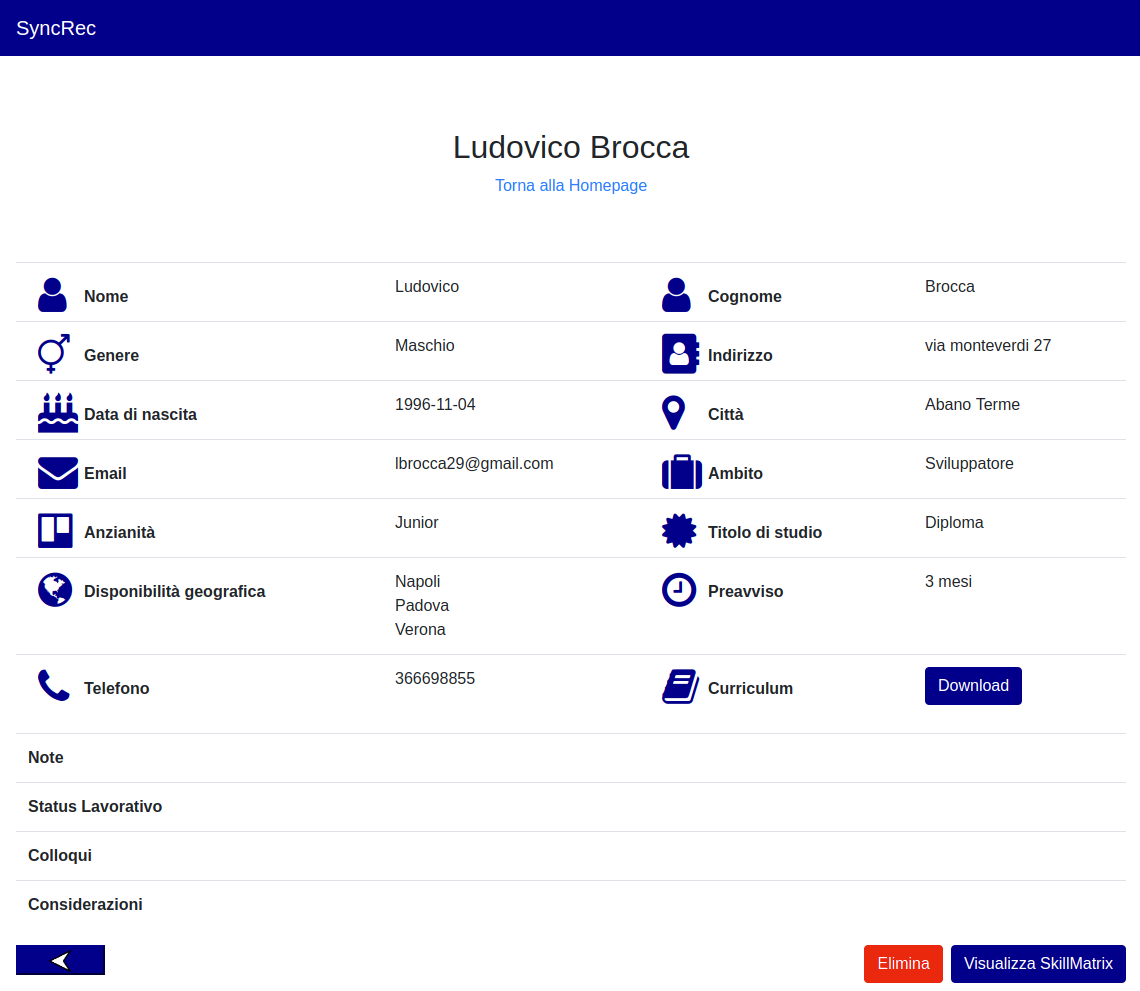
\includegraphics[width=1\columnwidth]{immagini/svil/applicant}
	\caption{Maschera CRUD del singolo applicant}
	\label{figura:applicant}
\end{figure}

\vspace{0.5em}
\begin{figure}[!h] 
	\centering 
	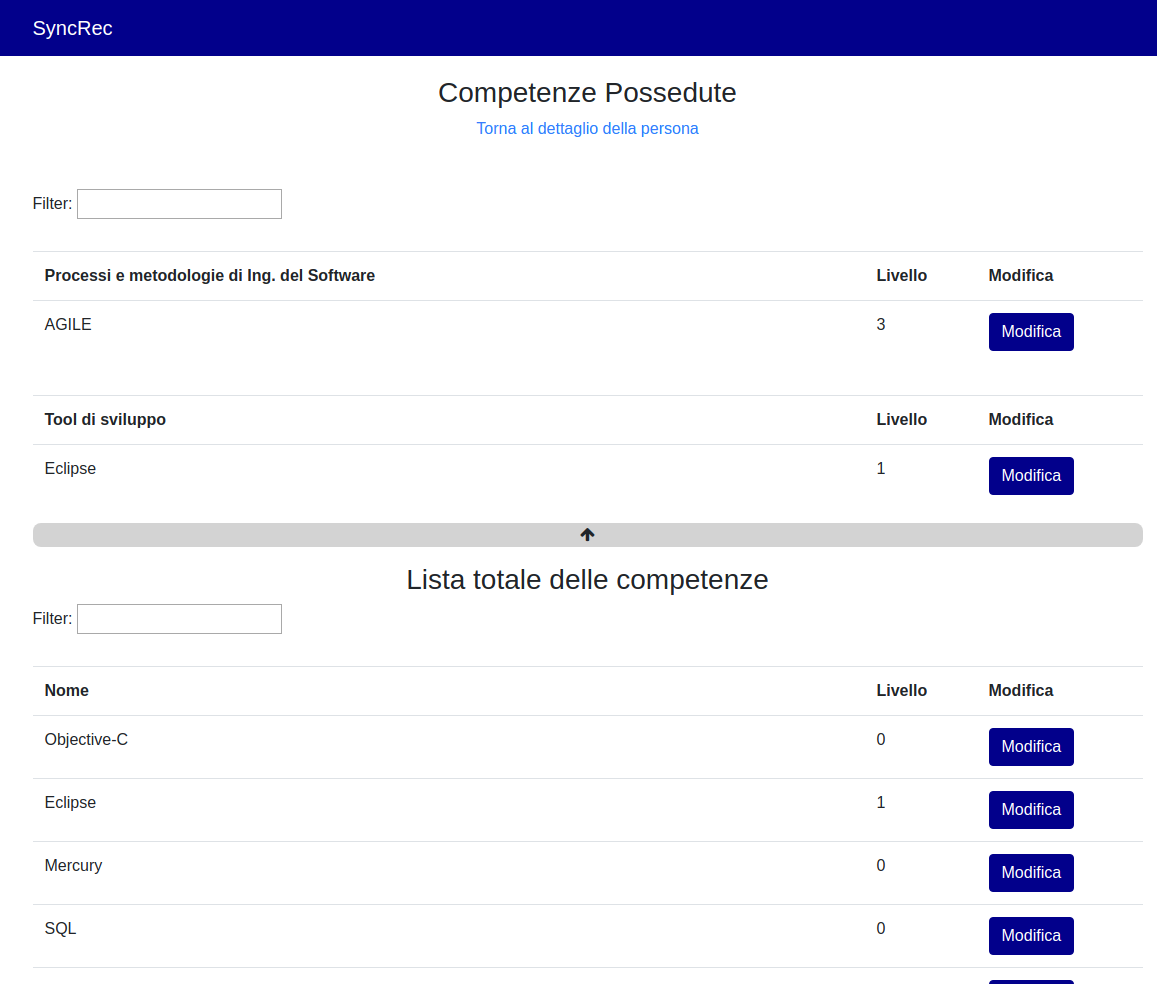
\includegraphics[width=1\columnwidth]{immagini/svil/skillmatrix} 
	\caption{Maschera CRUD dello skillmatrix}
	\label{figura:skillmatrix}
\end{figure}


\subsection{Sviluppo}
%Diagramma delle classi da fare qui%